% !TEX root = task-1-1-8.tex
% Editable task bank. Append new BankTask blocks at the end of the document.
\documentclass[12pt,a4paper]{article}
\usepackage{physics-textbook}
\usepackage{graphicx,needspace}
\usetikzlibrary{decorations.pathmorphing}
\newif\ifShowSolutions
\ifdefined\TutorEdition
  \ShowSolutionstrue
\else
  \ShowSolutionsfalse % Change to \ShowSolutionstrue to display solutions.
\fi
\newcounter{banktask}
\newsavebox{\BankTaskBox}
\newcommand{\BankTaskContent}[3]{%
  \noindent\textbf{\thebanktask.}\quad #2\par
  \ifShowSolutions
    \Needspace{50mm}% Keep the solution heading with its opening text or diagram.
    #3\par
    \ifdefined\TutorEdition
      \ifcsname TutorSource#1\endcsname
        \nopagebreak\smallskip{\small\csname TutorSource#1\endcsname\par}%
      \fi
    \fi
  \fi
}
\newcommand{\BankTask}[3]{%
  \refstepcounter{banktask}\par\medskip
  \sbox{\BankTaskBox}{\begin{minipage}{\linewidth}%
    \BankTaskContent{#1}{#2}{#3}\end{minipage}}%
  \ifdim\dimexpr\ht\BankTaskBox+\dp\BankTaskBox\relax>\dimexpr\textheight-20mm\relax
    \Needspace{35mm}\BankTaskContent{#1}{#2}{#3}%
  \else
    \Needspace{\dimexpr\ht\BankTaskBox+\dp\BankTaskBox\relax}%
    \noindent\usebox{\BankTaskBox}\par
  \fi
  \medskip
}
\begin{document}
\BookSubsection{1.1.8}{Закон сложения скоростей}


% Source sdamgia-317: https://phys-ege.sdamgia.ru/problem?id=317
\BankTask{sdamgia-317}{
Пловец плывет по течению реки. Определите скорость пловца относительно берега, если скорость пловца относительно воды $0{,}4\,\text{м/с}$, а скорость течения реки $0{,}3\,\text{м/с}$. (Ответ дайте в метрах в секунду.)
}{
\smallskip\noindent\textbf{Решение}\par
Вектор скорости пловца относительно берега есть сумма векторов скорости пловца относительно воды и скорости течения реки: $\vec v_{\text{пл–бер}}=\vec v_{\text{пл–вода}}+\vec v_{\text{вода}}.$ Поскольку пловец плывет по течению реки, получаем, что для величин скоростей выполняется соотношение: $v_{\text{пл–бер}}=v_{\text{пл–вода}}+v_{\text{вода}}=0{,}4\,\text{м/с}+0{,}3\,\text{м/с}=0{,}7\,\text{м/с}.$

Ответ: $0{,}7$.
}

% Source sdamgia-126: https://phys-ege.sdamgia.ru/problem?id=126
\BankTask{sdamgia-126}{
Два автомобиля движутся по прямому шоссе: первый — со скоростью $\vec v ,$ второй — со скоростью $( - 3\vec v ) .$ Какова скорость второго автомобиля относительно первого?

$1$) $\vec v$

$2$) $- 4\vec v$

$3$) $- 2\vec v$

$4$) $4\vec v$
}{
\smallskip\noindent\textbf{Решение}\par
Скорость второго автомобиля относительно первого равна $\vec v _2 - \vec v _1= - 3\vec v - \vec v = - 4\vec v .$

Ответ: $2$.
}

% Source sdamgia-3549: https://phys-ege.sdamgia.ru/problem?id=3549
\BankTask{sdamgia-3549}{
Пароход движется по реке против течения со скоростью $5\,\text{м/с}$ относительно берега. Определите скорость течения реки, если скорость парохода относительно берега при движении в обратном направлении равна $8\,\text{м/с}$. (Ответ дайте в метрах в секунду.)
}{
\smallskip\noindent\textbf{Решение}\par
Обозначим искомую скорость течения реки через $u$, а скорость парохода в стоячей воде — через $v .$ Тогда можно составить следующие уравнения. Скорость парохода вниз по течению равна $v + u=8\,\text{м/с}.$ Скорость парохода вверх по течению: $v - u=5\,\text{м/с}.$ Решая систему из двух этих уравнений, для скорости течения воды имеем $u=1{,}5\,\text{м/с}.$

Ответ: $1{,}5$.
}

% Source sdamgia-6038: https://phys-ege.sdamgia.ru/problem?id=6038
\BankTask{sdamgia-6038}{
Мотоцикл едет по прямой дороге с постоянной скоростью $50\,\text{км/ч}$. По той же дороге навстречу ему едет автомобиль с постоянной скоростью $70\,\text{км/ч}$. Чему равен модуль скорости движения мотоцикла относительно автомобиля? (Ответ дайте в километрах в час.)
}{
\smallskip\noindent\textbf{Решение}\par
Перейдем в систему отсчета, связанную с автомобилем. Модуль скорости движения мотоцикла в данной системе отсчета будет равен $50 + 70 = 120\,\text{км/ч}$.

Ответ: $120$.
}

% Source sdamgia-3548: https://phys-ege.sdamgia.ru/problem?id=3548
\BankTask{sdamgia-3548}{
Пешеход идет по прямолинейному участку дороги со скоростью $4\,\text{км/ч}$. Навстречу ему движется автобус со скоростью $40\,\text{км/ч}$. С какой скоростью (в км/ч) должен двигаться навстречу пешеходу велосипедист, чтобы модуль его скорости относительно пешехода и автобуса был одинаков?
}{
\smallskip\noindent\textbf{Решение}\par
Обозначим искомую скорость велосипедиста через $v .$ Тогда, как видно из рисунка, велосипедист приближается к пешеходу со скоростью $v + 4,$ а к автобусу — со скоростью $40 - v .$

\begin{center}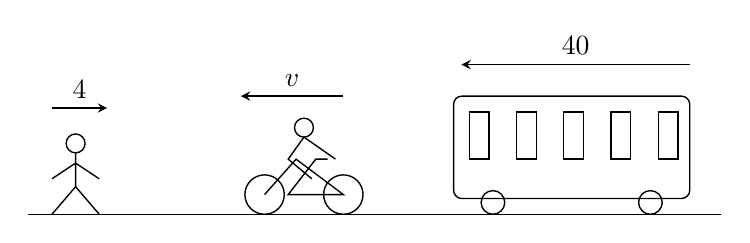
\begin{tikzpicture}[>=stealth,line width=.5pt]

\draw(-.4,0)--(8.4,0);
\draw(.2,.9)circle(.12);\draw(.2,.78)--(.2,.35)--(-.1,0) (.2,.35)--(.5,0) (.2,.65)--(-.1,.45) (.2,.65)--(.5,.45);
\draw[->](-.1,1.35)--(.6,1.35)node[midway,above]{$4$};
\draw(2.6,.25)circle(.25) (3.6,.25)circle(.25);\draw(2.6,.25)--(3,.7)--(3.6,.25)--(2.9,.25)--(3.25,.7)--(3.4,.7);\draw(3.1,1.1)circle(.12);\draw(3.1,.98)--(2.9,.7)--(3.2,.45) (3.1,.98)--(3.5,.7);
\draw[->](3.6,1.5)--(2.3,1.5)node[midway,above]{$v$};
\draw[rounded corners=3pt](5,.2)rectangle(8,1.5);\foreach\x in{5.2,5.8,6.4,7,7.6}\draw(\x,.7)rectangle(\x+.25,1.3);\draw(5.5,.15)circle(.15) (7.5,.15)circle(.15);
\draw[->](8,1.9)--(5.1,1.9)node[midway,above]{$40$};
\end{tikzpicture}\end{center}

Приравняв эти две скорости, находим требуемую скорость велосипедиста: $v + 4=40 - v \Longleftrightarrow  v =18\,\text{км/ч}.$

Ответ: $18$.
}

% Source sdamgia-131: https://phys-ege.sdamgia.ru/problem?id=131
\BankTask{sdamgia-131}{
Лодка должна попасть на противоположный берег реки по кратчайшему пути в системе отсчета, связанной с берегом. Скорость течения реки $u$, а скорость лодки относительно воды $v .$ Чему должен быть равен модуль скорости лодки относительно берега?

$1$) $v + u$

$2$) $v - u$

$3$) $\sqrt{v^2+u^2}$

$4$) $\sqrt{v^2-u^2}$
}{
\smallskip\noindent\textbf{Решение}\par

\begin{center}\begin{tikzpicture}[>=stealth,line width=.5pt]

\draw[->,thick](0,2)--(2,2)node[midway,above]{$\vec u_{\text{вод}}$};\draw[->,thick](2,0)--(0,2)node[midway,left]{$\vec v_{\text{лод–вод}}$};\draw[->,thick](2,0)--(2,2)node[midway,right]{$\vec v_{\text{лод–бер}}$};
\end{tikzpicture}\end{center}
$1$ способ:

По закону сложения скоростей, вектор скорости лодки относительно берега (неподвижной с. о.) равен сумме скорости лодки относительно воды (подвижной с. о.) и скорости течения воды (переносной скорости). По условию, вектор скорости лодки в системе отсчета, связанной с берегом, должен быть перпендикулярен ему. Построив «треугольник скоростей» из теоремы Пифагора для скорости лодки относительно берега имеем

\[v_\bot=\sqrt{v^2-v_\parallel^2}=\sqrt{v^2-u^2}.\]

$2$ способ:

\begin{center}\begin{tikzpicture}[>=stealth,line width=.5pt]

\draw[thick](0,0)--(5,0) (0,2.4)--(5,2.4);\node[above]at(.5,2.4){берег};\node[below]at(.5,0){берег};\node at(.5,1.1){река};\draw[->](.2,1.8)--(1.2,1.8)node[midway,above]{$u$};
\draw[dashed](2,0)--(2,1.7)--(3,1.7);\draw[->](3,0)--(2,0)node[midway,below]{$v_\parallel$};\draw[->](3,0)--(2,1.7)node[midway,left]{$v$};\draw[->](3,0)--(3,1.7)node[midway,right]{$v_\bot=\sqrt{v^2-v_\parallel^2}$};
\end{tikzpicture}\end{center}
Вектор скорости лодки относительно воды разложим на две компоненты: $\vec v =\vec v _\parallel + \vec v _\bot,$ где вектор $\overrightarrow v _\parallel$ направлен параллельно берегу, а вектор $\vec v _\bot$ — перпендикулярно берегу. Для того, чтобы лодка в системе отсчета, связанной с берегом, двигалась перпендикулярно к нему, необходимо, чтобы компонента скорости лодки относительно воды вдоль реки $v _\parallel$ в точности компенсировала скорость течения $u$. Тогда модуль скорости лодки относительно берега будет равен (по теореме Пифагора)

\[v_\bot=\sqrt{v^2-v_\parallel^2}=\sqrt{v^2-u^2}.\]

Ответ: $4$.
}

% Source sdamgia-11807: https://phys-ege.sdamgia.ru/problem?id=11807
\BankTask{sdamgia-11807}{
Расстояние между пунктами А и В равно $30\,\text{км}$. Из пункта А в направлении пункта В выезжает мотоциклист со скоростью $50\,\text{км/ч}$. Одновременно из пункта В в том же направлении, что и мотоциклист, выезжает трактор со скоростью $20\,\text{км/ч}$. На каком расстоянии от пункта А мотоциклист догонит трактор? Ответ приведите в километрах.
}{
\smallskip\noindent\textbf{Решение}\par
Для того чтобы догнать трактор, мотоциклисту нужно сократить расстояние в $30\,\text{км}$. Относительная скорость мотоциклиста относительно трактора равна $50\,\text{км/ч} - 20\,\text{км/ч} = 30\,\text{км/ч}$. Следовательно, мотоциклист догонит трактор за $\frac{30\,\text{км}}{30\,\text{км/ч}} = 1\,\text{ч}.$ За это время мотоциклист проедет $50\,\text{км}$.

Ответ: $50$.
}

% Source sdamgia-2915: https://phys-ege.sdamgia.ru/problem?id=2915
\BankTask{sdamgia-2915}{
В безветренную погоду самолет затрачивает на перелет между городами $6\,\text{часов}$. Если во время полета дует постоянный боковой ветер перпендикулярно линии полета, то самолет затрачивает на перелет на $9$ минут больше. Найдите скорость ветра, если скорость самолета относительно воздуха постоянна и равна $328\,\text{км/ч}.$
}{
\smallskip\noindent\textbf{Решение}\par
Путь, пройденный самолетом в первом случае: $s=v_{\text{СВ}}t_1,$ где $v_{\text{СВ}}$ — скорость самолета относительно воздуха. 

\begin{center}\begin{tikzpicture}[>=stealth,line width=.5pt]

\node at(-.3,.15){I};\draw[dashed](0,0)--(3.5,0);\draw[->](.8,0)--(2.3,0)node[midway,above]{$\vec v_{\text{СВ}}$};
\begin{scope}[xshift=4.6cm]\node at(-.3,.15){II};\draw[dashed](0,0)--(3.5,0);\draw[->](.2,0)--(2.8,0)node[midway,below]{$\vec v_{\text{С}}$};\draw[->](.2,0)--(.2,1)node[left]{$\vec v_{\text{В}}$};\draw[->](.2,1)--(2.8,0)node[midway,above]{$\vec v_{\text{СВ}}$};\end{scope}
\end{tikzpicture}\end{center}

Закон сложения скоростей в векторном виде для перелета во время ветра: $\vec v_{\text{С}}=\vec v_{\text{СВ}}+\vec v_{\text{В}},$ где $\vec v_{\text{В}}$ — скорость ветра. Выражение для модуля скорости самолета относительно Земли во втором случае имеет вид: 

\[v_{\text{С}}=\sqrt{v_{\text{СВ}}^2-v_{\text{В}}^2}.\]

Тогда путь, пройденный самолетом во втором случае:

\[s=v_{\text{С}}t_2=\sqrt{v_{\text{СВ}}^2-v_{\text{В}}^2}\,t_2.\]

Следовательно: 

$v_{\text{СВ}}t_1=\sqrt{v_{\text{СВ}}^2-v_{\text{В}}^2}\,t_2.$ Отсюда: 

\[v_{\text{В}}=\frac{v_{\text{СВ}}\sqrt{t_2^2-t_1^2}}{t_2}.\]

Ответ: $v _B=72\,\text{км/ч}=20\,\text{м/с}.$
}

% Source sdamgia-9752: https://phys-ege.sdamgia.ru/problem?id=9752
\BankTask{sdamgia-9752}{
Скорость течения широкой реки $3{,}6\,\text{км/ч}$. Под каким углом к направлению течения реки лодочник должен направлять лодку, скорость которой относительно воды равна $2\,\text{м/с}$, чтобы за $15$ минут ее снесло по направлению течения на $1{,}8\,\text{км}$?
}{
\smallskip\noindent\textbf{Решение}\par
При движении под углом $\alpha $ к течению реки, лодка будет двигаться по реке со скоростью 

\[V=V_{\text{теч}}+V_{\text{л}}\cos\alpha=3{,}6\cdot\frac{1000}{3600}+2\cos\alpha=(1+2\cos\alpha)\,\text{м/с}.\]

Тогда за время $t$ лодка переместится на расстояние

\[S=Vt= ( 1 + 2 \cdot  \cos  \alpha  ) t,\]

откуда

\[\cos  \alpha  = \frac{\frac{S}{t} - 1}{2} = \frac{1}{2} ( \frac{1800}{900} - 1 ) = \frac{1}{2} .\]

Лодочник должен направлять лодку под углом $60^\circ$ к направлению реки.

Ответ: $60$.
}

% Source sdamgia-23251: https://phys-ege.sdamgia.ru/problem?id=23251
\BankTask{sdamgia-23251}{
Школьник, возвращаясь домой с занятий по подготовке к ЕГЭ по физике, сел на вокзале в стоящую электричку. В это время пошел сильный снег, и вдоль поезда начал дуть ветер с постоянной скоростью. При этом поток падающих за окном снежинок выглядел так, как показано на рис. $1$. Потом поезд поехал, и после его разгона наблюдаемая через окно картина изменилась (см. рис. $2$). Углы наклона к горизонту прямолинейных траекторий снежинок в первом и во втором случаях были равны $\alpha  = 45 ^\circ$ и $\beta  = 10 ^\circ.$ С какой скоростью ехал поезд, если снежинки падают в неподвижном воздухе со скоростью $V = 1\,\text{м/с}$, электричка едет прямолинейно, а скорость и направление ветра не изменяются?
\begin{center}\begin{tikzpicture}[>=stealth,line width=.5pt]

\foreach\shift/\angle/\label in{0/45/1,5/10/2}{\begin{scope}[xshift=\shift cm]\draw(0,0)rectangle(4,3);\foreach\x in{.5,1.2,1.9,2.6,3.3}\foreach\y in{.4,1,1.6,2.2,2.8}\draw(\x,\y)--++(\angle:.15);\draw[thin](1.1,1.5)--(3,1.5);\draw[->,thick](2.6,1.5)--++(180+\angle:1.2);\draw(2.15,1.5)arc(180:180+\angle:.45);\node[below]at(2,-.15){Рис.\ \label};\end{scope}}
\node at(1.9,1.25){$\alpha$};\node at(6.9,1.23){$\beta$};
\end{tikzpicture}\end{center}

}{
\smallskip\noindent\textbf{Решение}\par
$1$. В неподвижной системе отсчета, связанной со стоящим поездом (рис. $1$), скорость снежинок $\overrightarrow V$ по закону сложения скоростей в кинематике складывается из двух составляющих — скорости $\overrightarrow V$ падения снежинки по вертикали и горизонтальной скорости ветра $\vec V_{\text{в}}:\quad\vec V_1=\vec V+\vec V_{\text{в}}.$ Поскольку векторы $\overrightarrow V$ и $\overrightarrow V_{\text{в}}$ взаимно перпендикулярны, а суммарный вектор $\overrightarrow V_1$ наклонен под углом $\alpha  = 45 ^\circ$ к горизонту, то модули $\overrightarrow V$ и $\overrightarrow V_{\text{в}}$ одинаковы и равны $V_{\text{в}}$ = $V = 1\,\text{м/с}$ — ветер дует влево с горизонтальной скоростью $1\,\text{м/с}$.

$2$. В системе отсчета, движущейся вместе с поездом (рис. $2$), снежинки приобретают относительно него дополнительную горизонтальную скорость $V_{\text{п}}$, направленную также влево (против вектора скорости поезда $\overrightarrow V_{\text{п}}$) и складывающуюся со скоростью ветра.

$3$. При этом вертикальная составляющая скорости снежинок остается равной $V = 1\,\text{м/с}$. Таким образом, как следует из прямоугольного треугольника для сложения горизонтальной и вертикальной составляющих скорости снежинки относительно поезда, $V = ( V_{\text{п}} + V_{\text{в}} ) \cdot  \tan  \beta  ,$ откуда $V_{\text{п}}=V/\tan\beta-V_{\text{в}}\approx1/0{,}176-1\approx4{,}67\,\text{м/с}\approx17\,\text{км/ч}.$

Ответ: $V_{\text{п}}\approx17\,\text{км/ч}.$
}


% Source 38F045: https://ege.fipi.ru/bank/questions.php?search=1&proj=BA1F39653304A5B041B656915DC36B38&qid=38F045
\BankTask{38F045}{
Из двух городов навстречу друг другу с постоянной скоростью движутся два автомобиля. На графике показано изменение расстояния между автомобилями с течением времени. С какой скоростью едет по дороге второй автомобиль, если скорость первого автомобиля равна $15\,\text{м}/\text{с}$? Скорость выразите в $\text{м}/\text{с}$.
\begin{center}
\begin{tikzpicture}[x=0.04cm,y=0.02cm,>=stealth]
\draw[->] (0,0)--(151,0) node[right] {$t,\,\text{мин.}$};
\draw[->] (0,0)--(0,181) node[above] {$S,\,\text{км}$};
\draw (0,144)--(30,144) (55,144)--(80,144) (105,144)--(120,144);
\draw (120,8)--(120,34) (120,83)--(120,132);
\draw[very thick] (0,144)--(60,0)--(120,144);
\node[below left] at (0,0) {$0$};
\node[left] at (0,144) {$144$};
\node[below] at (60,0) {$60$};
\node[below] at (120,0) {$120$};
\end{tikzpicture}
\end{center}
}{
\smallskip\noindent\textbf{Решение от GPT}\par
До встречи расстояние $144\,\text{км}$ уменьшается до нуля за $60\,\text{мин}=3600\,\text{с}$. Скорость сближения $v_1+v_2=\dfrac{144000}{3600}=40\,\text{м}/\text{с}$. Следовательно, $v_2=40-15=25\,\text{м}/\text{с}$.
}

% Source 5E532C: https://ege.fipi.ru/bank/questions.php?search=1&proj=BA1F39653304A5B041B656915DC36B38&qid=5E532C
\BankTask{5E532C}{
Расстояние между пунктами $A$ и $B$ равно $30\,\text{км}$. Из пункта $A$ в направлении пункта $B$ выезжает мотоциклист со скоростью $50\,\text{км}/\text{ч}$. Одновременно из пункта $B$ в том же направлении, что и мотоциклист, выезжает трактор со скоростью $20\,\text{км}/\text{ч}$. На каком расстоянии от пункта $A$ мотоциклист догонит трактор? Результат выразите в $\text{км}$.
}{
\smallskip\noindent\textbf{Решение от GPT}\par
Скорость сближения $v_{\text{отн}}=50-20=30\,\text{км}/\text{ч}$. Время $t=30/30=1\,\text{ч}$; от пункта $A$ мотоциклист проедет $s=50\cdot1=50\,\text{км}$.
}

% Source 424A13: https://ege.fipi.ru/bank/questions.php?search=1&proj=BA1F39653304A5B041B656915DC36B38&qid=424A13
\BankTask{424A13}{
Из населённого пункта одновременно в одном направлении выезжают грузовой автомобиль и бульдозер и движутся по дороге с постоянными скоростями. На графике показана зависимость расстояния между грузовиком и бульдозером от времени. Скорость грузовика равна $25\,\text{м}/\text{с}$, а скорость бульдозера меньше. С какой скоростью движется бульдозер? Результат выразите в $\text{м}/\text{с}$.
\begin{center}
\begin{tikzpicture}[x=0.065cm,y=0.055cm,>=stealth]
\draw[thin,dashed] (0,27)--(30,27) (30,0)--(30,27) (0,54)--(60,54) (60,0)--(60,54);
\draw[->] (0,0)--(90,0) node[right] {$t,\,\text{мин}$};
\draw[->] (0,0)--(0,81) node[above] {$S,\,\text{км}$};
\node[below] at (0,0) {$0$};
\node[below] at (30,0) {$30$};
\node[below] at (60,0) {$60$};
\node[left] at (0,27) {$27$};
\node[left] at (0,54) {$54$};
\draw[very thick] (0,0)--(60,54);
\end{tikzpicture}
\end{center}
}{
\smallskip\noindent\textbf{Решение от GPT}\par
Расстояние увеличивается со скоростью $54\,\text{км}/60\,\text{мин}=15\,\text{м}/\text{с}$. Поэтому $v_{\text{б}}=v_{\text{гр}}-15=25-15=10\,\text{м}/\text{с}$.
}

\end{document}
